\documentclass{beamer}
\usepackage{etex} % fixes new-dimension error
\usepackage{lmodern}
\usepackage[T1]{fontenc}
\usetheme{metropolis}
\metroset{block=fill}
%\usetheme{Boadilla}

\setbeamertemplate{footline}
{
  \leavevmode%
  \hbox{%
  \begin{beamercolorbox}[wd=.4\paperwidth,ht=2.25ex,dp=1ex,center]{author in head/foot}%
    \usebeamerfont{author in head/foot}\insertshortauthor
  \end{beamercolorbox}%
  \begin{beamercolorbox}[wd=.5\paperwidth,ht=2.25ex,dp=1ex,center]{title in head/foot}%
    \usebeamerfont{title in head/foot}\insertsection
  \end{beamercolorbox}%
  \begin{beamercolorbox}[wd=.1\paperwidth,ht=2.25ex,dp=1ex,right]{date in head/foot}%
    \insertframenumber{} / \inserttotalframenumber\hspace*{2ex} 
  \end{beamercolorbox}}%
  \vskip0pt%
}
\makeatother
\setbeamertemplate{navigation symbols}{}
%----------------------------------------------------------------------------
\usepackage{graphicx,amsmath}
\usepackage{stmaryrd} % cf. interleave
\usepackage{booktabs}
\usepackage{amscd}
\usepackage{multicol}
\usepackage[absolute,overlay]{textpos}
\usepackage{alltt}
\usepackage{proof}
\usepackage{listings}
%------ using pstricks (rnode etc) ------------------------------------------
\usepackage{pstricks,pst-node,pst-text,pst-3d}

% ------ using color ---------------------------------------------------------
\newrgbcolor{goldenrod}{.80392 .60784 .11373}
\newrgbcolor{darkgoldenrod}{.5451 .39608 .03137}
\newrgbcolor{brown}{.15 .15 .15}
\newrgbcolor{darkolivegreen}{.33333 .41961 .18431}
\def\gold#1{{\goldenrod #1}}
\def\dgold#1{{\alert{#1}}}
\def\dkb#1{{\blue #1}}
\def\tdkb#1{\textbf{\darkblue #1}}
\def\gre#1{{\darkolivegreen #1}}
\def\gry#1{{\gray #1}}
\def\rdb#1{{\red #1}}
%----------------------------------------------------------------------------

\AtBeginSection[]
{
    \begin{frame}
        \frametitle{Table of Contents}
        \tableofcontents[currentsection]
    \end{frame}
}

\author[Renato Neves]{Renato Neves}

% logos of institutions
\titlegraphic{
  \begin{textblock*}{5cm}(6.5cm,7.4cm)
     
\includegraphics[scale=0.06]{images/uminho.png}\hspace*{.85cm}~%
  \end{textblock*}
  \begin{textblock*}{5cm}(9.2cm,7.45cm)
    
\includegraphics[scale=0.50]{images/haslab.pdf}
  \end{textblock*}
}

% No date
\date{}

\begin{document}

\title{Semantics of Programming Languages}

\frame[plain]{\titlepage}
\section{Motivation}
\begin{frame}{ The search for meaning }

  \begin{examples}
    \begin{itemize}
            \item $f()\{ \mathtt{prt}\ a; \> \mathtt{ret \ 1} \} ;\
                g()\{ \mathtt{prt}\ b; \> \mathtt{ret \ 0} \};\
                x:= f() \vee g()$
                \\[10pt]
            \item $x:=2\ ; (x := x + 1 \parallel  x := 0)$ 
                \\[10pt]
            \item $(a:= 1\, ; \mathtt{prt}\ b) \parallel 
                    (b:= 1\, ; \mathtt{prt}\ a)$ 
    \end{itemize}
  \end{examples}

  \vfill
  \pause
  \centering 
  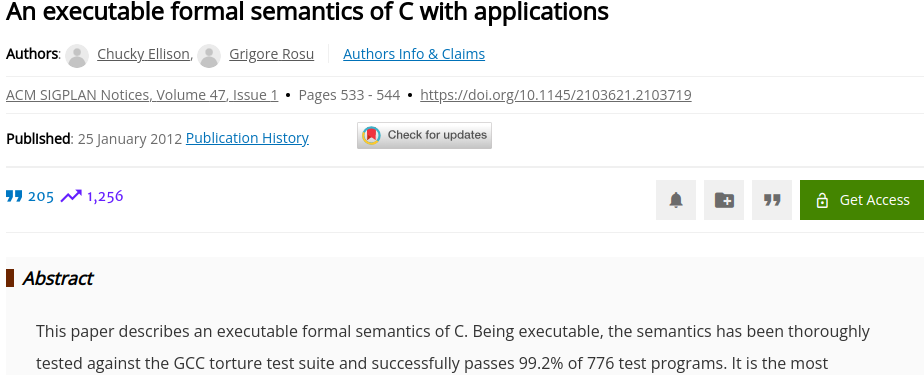
\includegraphics[scale=0.28]{images/c.png}
\end{frame}

\begin{frame}{ The search for meaning }
    \begin{examples}
    \begin{itemize}
            \item $\mathtt{p ; (q ; r)} \stackrel{?}{=} \mathtt{(p ; q) ; r} $
                    \\[10pt]
            \item $\mathtt{p \parallel q \stackrel{?}{=} q \parallel p} $ 
                    \\[10pt]
            \item $\mathtt{\left (p +_{\frac{1}{2}} q \right ) ; r 
                    \stackrel{?}{=} p ; r +_{\frac{1}{2}} q ; r}$ 
                    \\[10pt]
            \item $\mathtt{entangle(x,y) \stackrel{?}{=}}$ spooky action 
    \end{itemize}
  \end{examples}

  \pause
  \center
  \fbox{
  Will my program behave correctly ?
  }
\end{frame}

\lstset{ 
  basicstyle=\ttfamily\footnotesize,        % the size of the fonts that are used for the code
  breakatwhitespace=false,         % sets if automatic breaks should only happen at whitespace
  breaklines=true,                 % sets automatic line breaking
  deletekeywords={...},            % if you want to delete keywords from the given language
  escapeinside={\%*}{*)},          % if you want to add LaTeX within your code
  extendedchars=true,              % lets you use non-ASCII characters; for 8-bits encodings only, does not work with UTF-8
  keepspaces=true,                 % keeps spaces in text, useful for keeping indentation of code (possibly needs columns=flexible)
  keywordstyle=\color{blue},       % keyword style
  language=C,                 % the language of the code
  morekeywords={*,...},            % if you want to add more keywords to the set
  rulecolor=\color{black},         % if not set, the frame-color may be changed on line-breaks within not-black text (e.g. comments (green here))
  showstringspaces=false,          % underline spaces within strings only
  showtabs=false,                  % show tabs within strings adding particular underscores
  tabsize=2,	                   % sets default tabsize to 2 spaces
}

\begin{frame}[fragile]{A particle and its orbital trajectory -- what can go wrong?}
        \begin{lstlisting}
        x := -1; v := 0; a := 1;
        while true do {
	            if x <= 0 then a := 1; else a :=-1;
    	        x' = v, v' = a for 0.5;
        }
        \end{lstlisting}
        
        \pause
        \begin{center}
                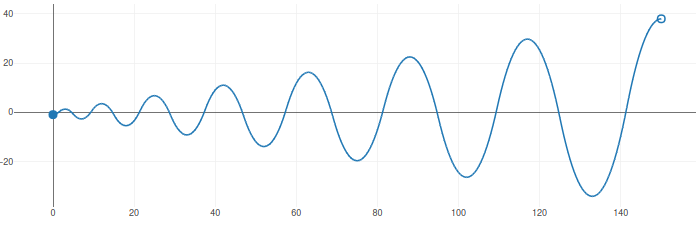
\includegraphics[scale=0.3]{images/lochness.png}
        \end{center}
\end{frame}

\begin{frame}{ The search for meaning }

  \begin{minipage}[1\textheight]{\textwidth}

  \begin{columns}[c]
  \begin{column}{0.7\textwidth}

        But\dots  what is a programming language really ?

        And what is computation ? 

  \end{column}
  \begin{column}{0.2\textwidth}
    
        
\includegraphics[scale=0.1]{images/hitchhiker.jpg}
  \end{column}
  \end{columns}
  \end{minipage}

  \vfill
  \pause
  To answer these questions we will turn programming into \alert{mathematics}
  \dots

  in the same way that (other?) natural phenomena are turned into mathematics
  (electromagnetism, quantum physics \dots)
\end{frame}

\section{Roadmap}

\begin{frame}{A sprinkle of linguistics}
  We will face two linguistic concepts that every programmer
  ought to know
  \begin{itemize}
  \item syntax - determines whether a sentence
    is valid or not
  \item semantics - the meaning of valid sentences
  \end{itemize}

  \vfill
  \begin{example}[syntax]
      The sentence (program) $\mathtt{x := p\, ;q}$ is forbidden by
      the syntactic rules of most programming languages
    \end{example}
  \begin{example}[semantics]
      The sentence (program) $\mathtt{x := 1}$ has the meaning ``writes
      \texttt{1} in the memory address corresponding to \texttt{x}''
  \end{example}
\end{frame}

\begin{frame}{Semantics for every season}

        \hspace*{+5pt}\makebox[\linewidth][c]{%
        \begin{tabular}{ l l }
        Operational semantics & \alert{How} a program operates
        \\
        Denotational semantics & \alert{What} a program mathematically is 
        \\
        Axiomatic semantics & \alert{Which} logical properties a program
        satisfies
        \end{tabular}
        }

        \vfill
        \pause
        Some truly surprising properties arise from their interaction \dots
\end{frame}

\begin{frame}{An apparently impossible program}

        Take a concurrent program $\mathtt{p}$

        It relies on an external scheduler to interleave its actions

        There are infinitely many schedulers even \alert{uncountably} many

        Yet one can write down a program that checks whether $\mathtt{p}$
        satisfies a given property \alert{for all} schedulers \dots\ in \alert{finite}
        time !!
\end{frame}

\begin{frame}{How deep will we go into the rabbit hole ?}

  \begin{minipage}[1\textheight]{\textwidth}
  \begin{columns}[c]
  \begin{column}{0.8\textwidth}

    Our learning path will intersect theory and practice,
  
    from the very basics to the state-of-the-art ---

    we will face current limitations and see what challenges lie ahead 

  \end{column}
  \begin{column}{0.2\textwidth}
    
  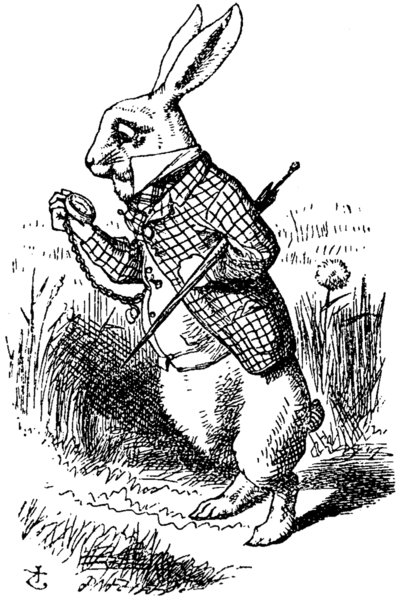
\includegraphics[scale=1.4]{images/rabbit.png}
  \end{column}
  \end{columns}
  \end{minipage}

\end{frame}

\section{Logistics}

\begin{frame}{Assessment}

  Two written tests (24 Mar and 26 May)

\end{frame}

\begin{frame}{Materials and Contacts}
  Relevant class material and announcements posted on the website

  \url{http://lmf.di.uminho.pt/SLP-2425/}

  e-mail: \href{mailto:nevrenato@di.uminho.pt}{nevrenato@di.uminho.pt}

  office hours: wednesday afternoon (please send an email the day before if you wish to meet)
\end{frame}

\nocite{winskel93,nielson07,crole03}
\bibliographystyle{amsalpha}
\bibliography{main.bib}
\end{document}
